\section{Method}
\label{method}
%TODO computer aided network analysis <- distinction between 'verkostotutkimus' mentioned in Juuso Marttila's thesis. 
My method is computer aided (social) network analysis. It is one of the most implemented methods in the field of digital humanities. Generally network analysis has other more everyday applications, such as, the analysis of the internet as a network in the field of technology. Quite a few textbooks have been written on network analysis.

%Furthermore, in the field of technology network analysis does have some everyday application, such as the analysis of the internet. 

\subsection{Defining the network}
Network analysis combines mathematics, statistics and social scineces. Primarily it is based on the mathematical graph theory. A graph is a representation of the network. Graph includes nodes (also colled vertice) and edges (also called links and connections).

\begin{figure}[h]
	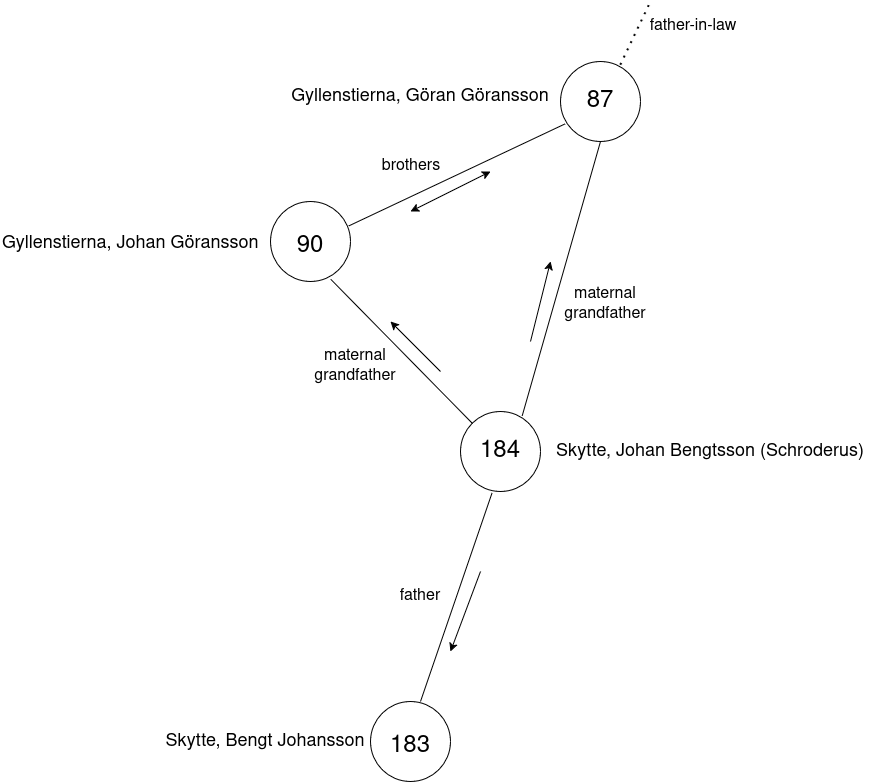
\includegraphics[scale=0.25]{example_network.drawio.png}
	\centering
	\caption{A sample from the graph} 
	\centering
\end{figure}
In this context the graph's nodes depict individual councillors with the input of name and id number. Correspondingly the edges represent the kinships between two nodes. For instance, in Figure 1 we can see that Johan Bengtsson (Schroderus) Skytte (id 184) is Bengt Johansson Skytte's (id 183) father and a maternal grandfather for Johan Göransson Gyllenstierna (id 90) and Göran Göransson Gyllenstierna (id 87). Johan Göransson and Göran Göransson are brothers, however, their father is not mentioned in the dataset. Göran Göransson also has further links in the network. \footfullcite{councillorsDS}

Calculating different statistics is a crucial part of the network analysis. One of the most important measures is the \textbf{node degree}. In all its simplicity node degree means the amount of edges connected to a specific node. For example, the degree of Johan Bengtsson (Schroderus) Skytte (id 184) is three or the degree of Bengt Johansson Skytte (id 183) is one. The \textbf{average degree} is the mean [keskiarvo] of all the node degrees of the specific graph. The \textbf{density} of the network is based on the node degrees. In very dense network almost every node is connected to each other, but a sparse graph has just a few edges in it.

Another important factor is whether the graph is \textbf{directed} or \textbf{undirected}. In directed graph the edges have directions, like in the communication networks a message has a sender and a receiver. The directions are marked with an arrow. In undirected graphs the edges are bidirectional (two way), for example, a relationship between two brothers can be understood as undirected. Directed graphs have more features and a more complex structures, for instance, the degrees of inbound and outbound edges can be counted separately. For sipmlicity, the graphs presented in this work are undirected.

\subsection{Implementation of the network analysis}
The data processing and analysis is conducted with a combination of Python programming language and Gephi software. Python is used for extracting the data from the councillors-dataset and formulating it in the right format: readable for Gephi. The actual network analysis, visualization and calculating statistics, is performed with Gephi. 

Python is a programming language popular amongst scientists. I selected Python due its simple syntax and ease in implementing small tasks like data processing. The language is understandable and widely used, which makes the work replicable. To be precise the script is written with Python 3.

As graphs are structures commonly used in programming, it would have been possible to conduct the actual network analysis using tools provided by Python, yet, Gephi software provides a visual user interface and more intuitive tools for the manipulation of the graph. Furthermore, the Gephi format makes the data and graph accessible also for non programmers.

Gephi is a software for network visualization and analysis. It contains tools for manipulating, filtering, clustering and visualizing the graph. It has built in appliances for fixing errors in data and calculating necessary statistics.\footcite{gephi} Gephi reads data from text format (comma separated values .csv) or Microsoft Excel tables (XLSX), and Gephi projects are saved as .gephi files. The processed graphs and data can be exported as images or tables.  

Nonetheless, Gephi does have some weaknesses. It is not always the most intuitive to use, and especially the visual configurations of the graph causes some issues. I have encountered difficulties with the node labels (the councilor's name next to the node). Sometimes the problems lies in the Gephi settings, but if the whole software crashes when trying to make the node labels visible, the problem lies within the software itself and should be solved when starting the program.\footnote{For Linux environments opening Gephi from command line with command "LIBGL\_ALWAYS\_SOFTWARE=1 ./gephi" can sometimes help.} 

Both of these tools are also open source and free to download. All scripts written for this work available on GitHub.\footnote{\url{https://github.com/Heidi-Suurkaulio/mastersthesis} TODO right link later}

Basically the steps of network analysis are : \begin{enumerate}
	\item Choosing the subject and data
	\item Pre processing the data for the network analysis
	\item Constructing the graph and finding possible issues and errors 
	\item Counting the statistics
	\item Deciding the layout (algorithm)
	\item Doing the interpretations
\end{enumerate}
However, the analysis is not that straightforward, sometimes the steps 2 and 3 must be repeated and re-repeated. Yet, on some circumstances the graph is not visualized or the statistics are not deemed important. These steps will be discussed in practice below.

\subsubsection{Test run}
%TODO fix councillor / councillor typo

To draft the structure of the graph and understand the nuances of the given data, a test run was carried out. The test run was done with a simple Python script, and no attention was paid to the temporal aspects of the network or the potential directions within the graph. The script and Gephi project used, and the visualization of the graph of the test run is available in GitHub in the TestRun folder\footnote{\url{https://github.com/Heidi-Suurkaulio/mastersthesis/tree/main/TestRun}}

The data processing was started by manually cleaning the data in LibreOffice Calc (equivalent to Microsoft Excel). The columns and rows containing information of the source material of the dataset and councillor's years active were removed. That made the structure of the data coherent and easier to manipulate with the Python script. The manually cleaned data is exported as .csv (comma separated values) file. The .csv file's header (the first line of the file) should be modified so that the column name "No." is changed to "Id" and "Family members in the council of the realm" is changed to "Family", the first one can cause an error if referenced in the Python code, the latter is inconveniently long.
%table 2

The script itself reads the data from the .csv file. The connections between the councillors are separated from the "Family" column, based on the knowledge that each connection is marked with the id number of another councillor. The connections are then formatted and printed to .csv file. The connections .csv file containing values for "Source" id of the source concillor, "Target" id of target councillor, "Type" standard "Undirected", "Id" id number for the connection, "Weight" standard 1.0. Another .csv file is formatted and printed with the information of councillors' names and id numbers.

\begin{table}[h]
	\caption{Example of the connections .csv file}
	\centering
	\begin{tabular}{cccccc}
		\hline
		1 &Source, &Target, &Type, &Id, &Weight \\
		\hline
		2 &231, &228, &Undirected, &0, &1.0 \\
		\hline
		3 &231, &230, &Undirected, &1, &1.0 \\
		\hline
	\end{tabular}
\end{table}
\begin{table}[h]
	\caption{Example of the councillors .csv file}
	\centering
	\begin{tabular}{ccc}	
		\hline
		1 &Id; &Label \\
		\hline
		2 &162; &Ingemar Petri \\
		\hline
		3 &231; &Tre Rosor, Ture Jönsson \\
		\hline
	\end{tabular}
\end{table}

These .csv files are readable for Gephi. The outcome was an undirected graph of the councillors' affiliation network that had accumulated during the 160 years. The graph consisted of 261 nodes (257 real + 4 "ghosts") and 372 edges (including self loops and "ghost" nodes). The test run revealed three problems within the graph: the emergence of the empty "ghost" nodes, parallel edges and thirdly self loops. 

The "ghost" nodes were excess nodes with no name and only an id number and one or two connections in the graph. They were due to the references to the data points removed from the original dataset, and therefore can be ignored. The ghosts are discussed further in the subsection \ref{sources}. However, the more essential problem were parallel edges and self loops.

The parallel edges occur because one relationship, such as father and son, is sometimes marked parallel in the dataset. For example, in the case of Göran Göransson Gyllenstierna (id 87) the relatives are "Maternal Grandfather 184, Brother 90, Father-in-law 3, ...", and the same relationship is found in his grandfather's Johan Bengtsson (Schroderus) Skytte's (id 184) links: "Son 183, Grandson through daughter 87". Yet, the connection to Göran Göransson's brother Johan Göransson Gyllenstierna (id 90) is not marked in the grandfathers links. This means that the node of Göran Göransson Gyllenstierna (id 87) has one excess link compared to his brother's node. The case is visualized in the Figure 2.

\begin{figure}[h]
	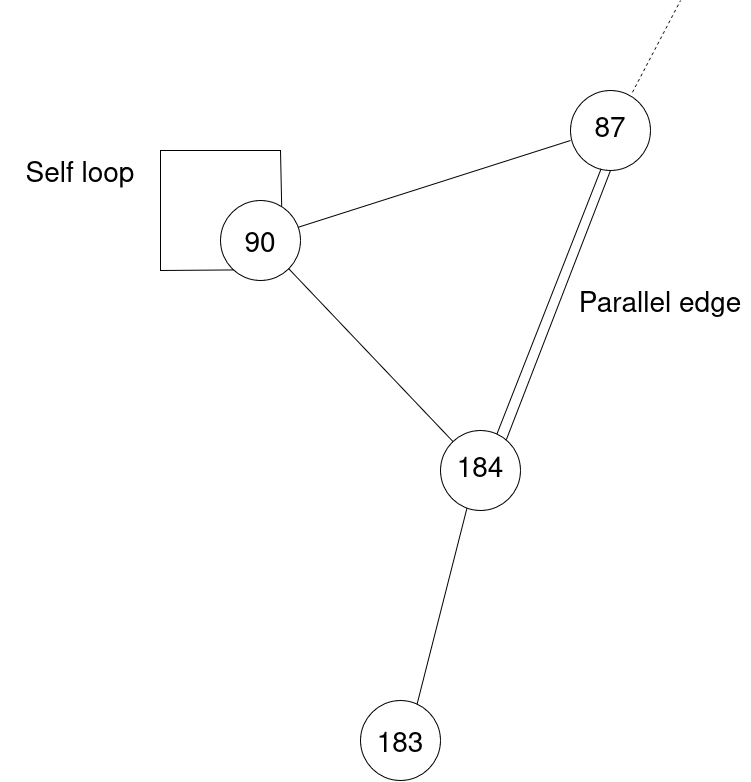
\includegraphics[scale=0.20]{double_link.drawio.png}
	\centering
	\caption{Visualisation of the parallel edge and self loop} 
	\centering
\end{figure}

These duplicate edges would cause bias to the calculation of the node degrees and any statistics based on them. A node degree is a sum of all the edges connected to one node, and if the relationships are inconsistently marked with one or two edges, the factually similar nodes would get different degrees. These inconsistent node degrees would accumulate when counting the average degrees an so forth. The problem of parallel edges is widely recognized in the field of network analysis, and therefore Gephi does have some builtin features for handling it.

While importing data to Gephi (on Import Spreadsheet) the strategy for merging the parallel edges can be chosen. One option is, for example, placing the sum or average of the parallel edges in the edge's degree, yet using only one connection to to represent the edge in the graph. In this context a more simple solution was chosen, with the option "Firs" Gephi will use only the first connection between two nodes ignoring any latter ones. This will reduce the amount of connections from 698 found in the connections.csv to only 372.

Self loops occur when one node has – for some reason or another – a connection to itself. Similarly to the parallel edges, they cause bias to the node degrees. In this graph a self loop can be found at least on the node with id 5 and id 90. In the case of id 5: Gustaf Axelsson Baner, his relatives are "Father 4, Father-in-law 217, Brother 9, Sons 5, 7, 8, 10, Sons-in-law 152 and 197", and similarly with id 90: Johan Göransson Gyllenstierna his family reads "Maternal Grandfather 184, Brother 90". These self loops are most likely caused by a typo in the dataset, because it is reasonable to assume that none is a son or brother to themselves.
 
Gephi does have a switch whether or not self loops are allowed in the graph, and it can automatically remove them based on the preference. The self loops are present in the test run graph alongside with the ghost nodes, yet those will be removed from the subsequent analysis. To highlight the ghosts they are colored cray, and the four nodes referred as an example here are colored red in the test run graph.

The last step in the preparation of the network analysis is the selection of the layout algorithm. For the test run an algorithm called Yifan Hu was used with default configurations except parameter theta set to 2.0. Then layout option "noOverlap" was chosen to separate possibly overlapping nodes, and some further manual placement of the nodes was done to make the graph more readable. The outcome was visually somewhat dense network in the middle and mostly unconnected isolated nodes around it. 

\subsection{Fitting modern model on historical timeperiod}
\begin{quote}
	Every model is an approximation.\\
	All models are wrong; some models are useful.\footcite[prefix]{statisticsfor}
\end{quote}

A graph is elementally a generalizing and simplifying model of complex social networks on the Swedish council of the Realm. Yet, when bulding any kinds of (computational) models, decisions between the complexity and abstraction must be made – in fact besides too simplifying models, too complex or overfitted ones are a problem on their own.\footcite{TODO} One of the most important question is what to include and and what to exclude. And, a more existential question is what we can model or even know about historical social networks. 

As I am working with pre-collected data, the choices have been made by the authors of the dataset Hakanen and Koskinen and by the scholars their work is leaning on. The data – and further the graph – is able to give a picture of the offically recorded family links within the council of the realm. However, it is not possible to know about the messy every day relationships, friendships, informal discussions, intentions, emotions or disputes these 257 men have had. It is important to understand the limitations of the data and model.

Generally, what comes to the study of early modern period, source material concerning women, lower social classes or marginalized groups are harder to find.\footcite{TODO} 
However, at least noble women are included in the contemporary lineage diagram as seen in figure \ref{queenlineage}. So maybe a network including noblewomen or the councilors patrons would be possible to build.

\begin{figure}
	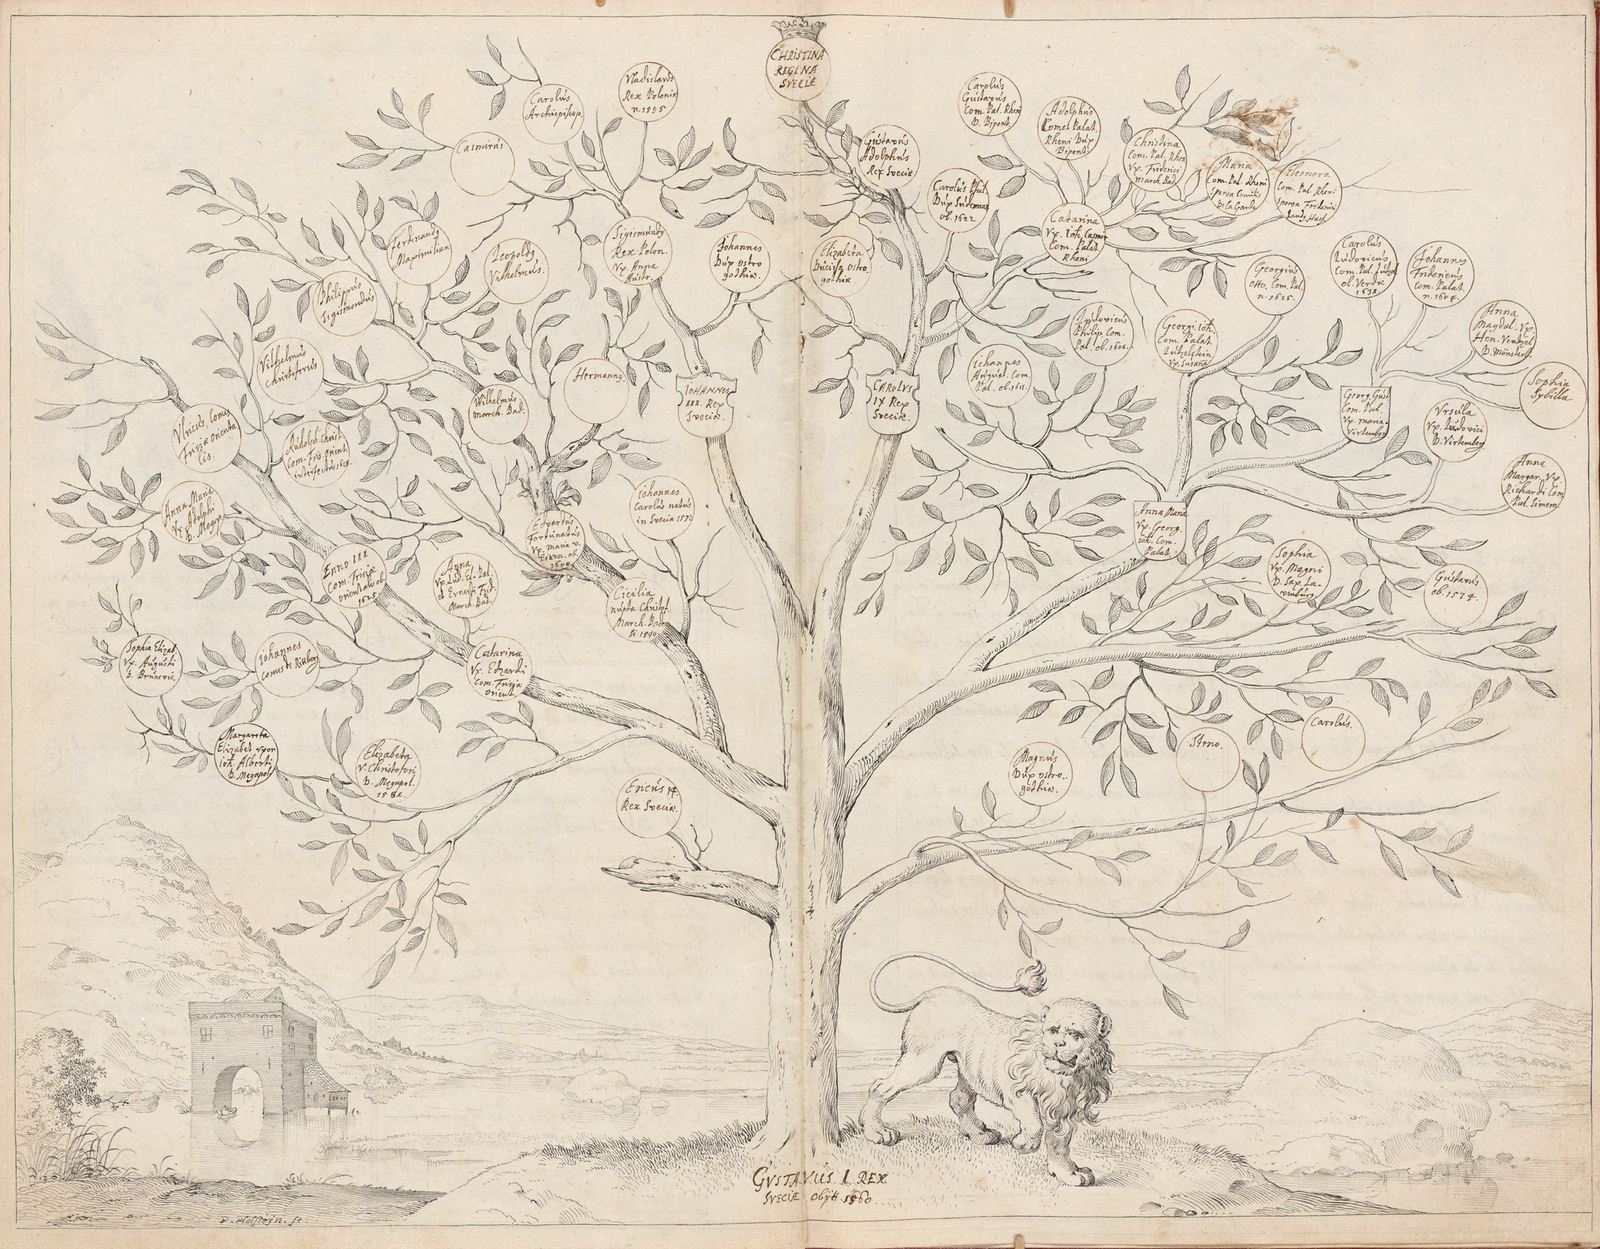
\includegraphics[width=\linewidth]{QueenChristinaLineage.png}
	\caption{Lineage of the house of Vasa from the \textit{Hortus Regius} or "Queen Christina's Genealogical Tree with Political Emblems".(\cite{hortusregius})} 
	\centering
	\label{queenlineage}
\end{figure}

It can be said with relative certainty that contemporaries in the early modern time didn't perceive their society as a network in the modern sense. And when studying ...
%TODO metonyme, biblical hierarchy, harmony
%TODO hopes and fears p. 21 - 22

For instance \textit{Hortus Regius} can be used as an illustration of the ideals and understandings of the early modern nobility. The book was given to queen Christina by a diplomat Shering Rosenhane in circa 1645, and it consists of delicately illustrated political emblems\footnote{Instructions, virtues, metaphors} and noble family trees leading to queen Christina.\footcite{congresslibrary} 
%TODO explain the lineage diagram
